\section{Results}

\subsection{Unitary Tests}

The individual software components and hardware drivers used in this project underwent rigorous \textbf{Unitary Testing} during the previous subject. These tests were essential to establish a verified baseline for the current system integration.

\subsection{Local Test}

A \textbf{Local Test} was performed to verify the integrity of the data acquisition and the preliminary encoding of the payload. As shown in \autoref{fig:local_feedback_test}, the system provides a comprehensive \textbf{Sensor Report} via the serial console, allowing for a side-by-side comparison between the raw sensor readings and the formatted \gls{LoRaWAN} values.

\begin{figure}[H]
    \centering
    \includegraphics[width=0.8\textwidth]{images/logs.png}
    \caption{\acrshort{LoRaWAN} Local Feedback Test}
    \label{fig:local_feedback_test}
\end{figure}

The confirmation message \textit{"Data packet sent successfully (30 bytes)"} indicates that the internal buffer has been correctly assembled and handed over to the \gls{LoRaWAN} stack for transmission to the ResIoT gateway.

\subsection{ResIoT Test}

The \textbf{ResIoT Test} focused on validating the LUA script responsible for decoding the incoming \gls{LoRaWAN} payloads. As shown in \autoref{fig:lua_test}, the test involved simulating an uplink message with a predefined hexadecimal payload and passing it through the LUA decoder function.

\begin{figure}[H]
    \centering
    \includegraphics[width=0.8\textwidth]{images/lua.png}
    \caption{LUA Test}
    \label{fig:lua_test}
\end{figure}

\subsection{System Integration Test}

The final validation of the project was conducted through a comprehensive \textbf{System Integration Test}, confirming the end-to-end functionality of the data pipeline, from physical sensing to cloud visualization. As shown in \autoref{fig:dashboard_test}, the \textbf{ResIoT Dashboard} successfully aggregates all telemetry streams into a cohesive monitoring station.

\begin{figure}[H]
    \centering
    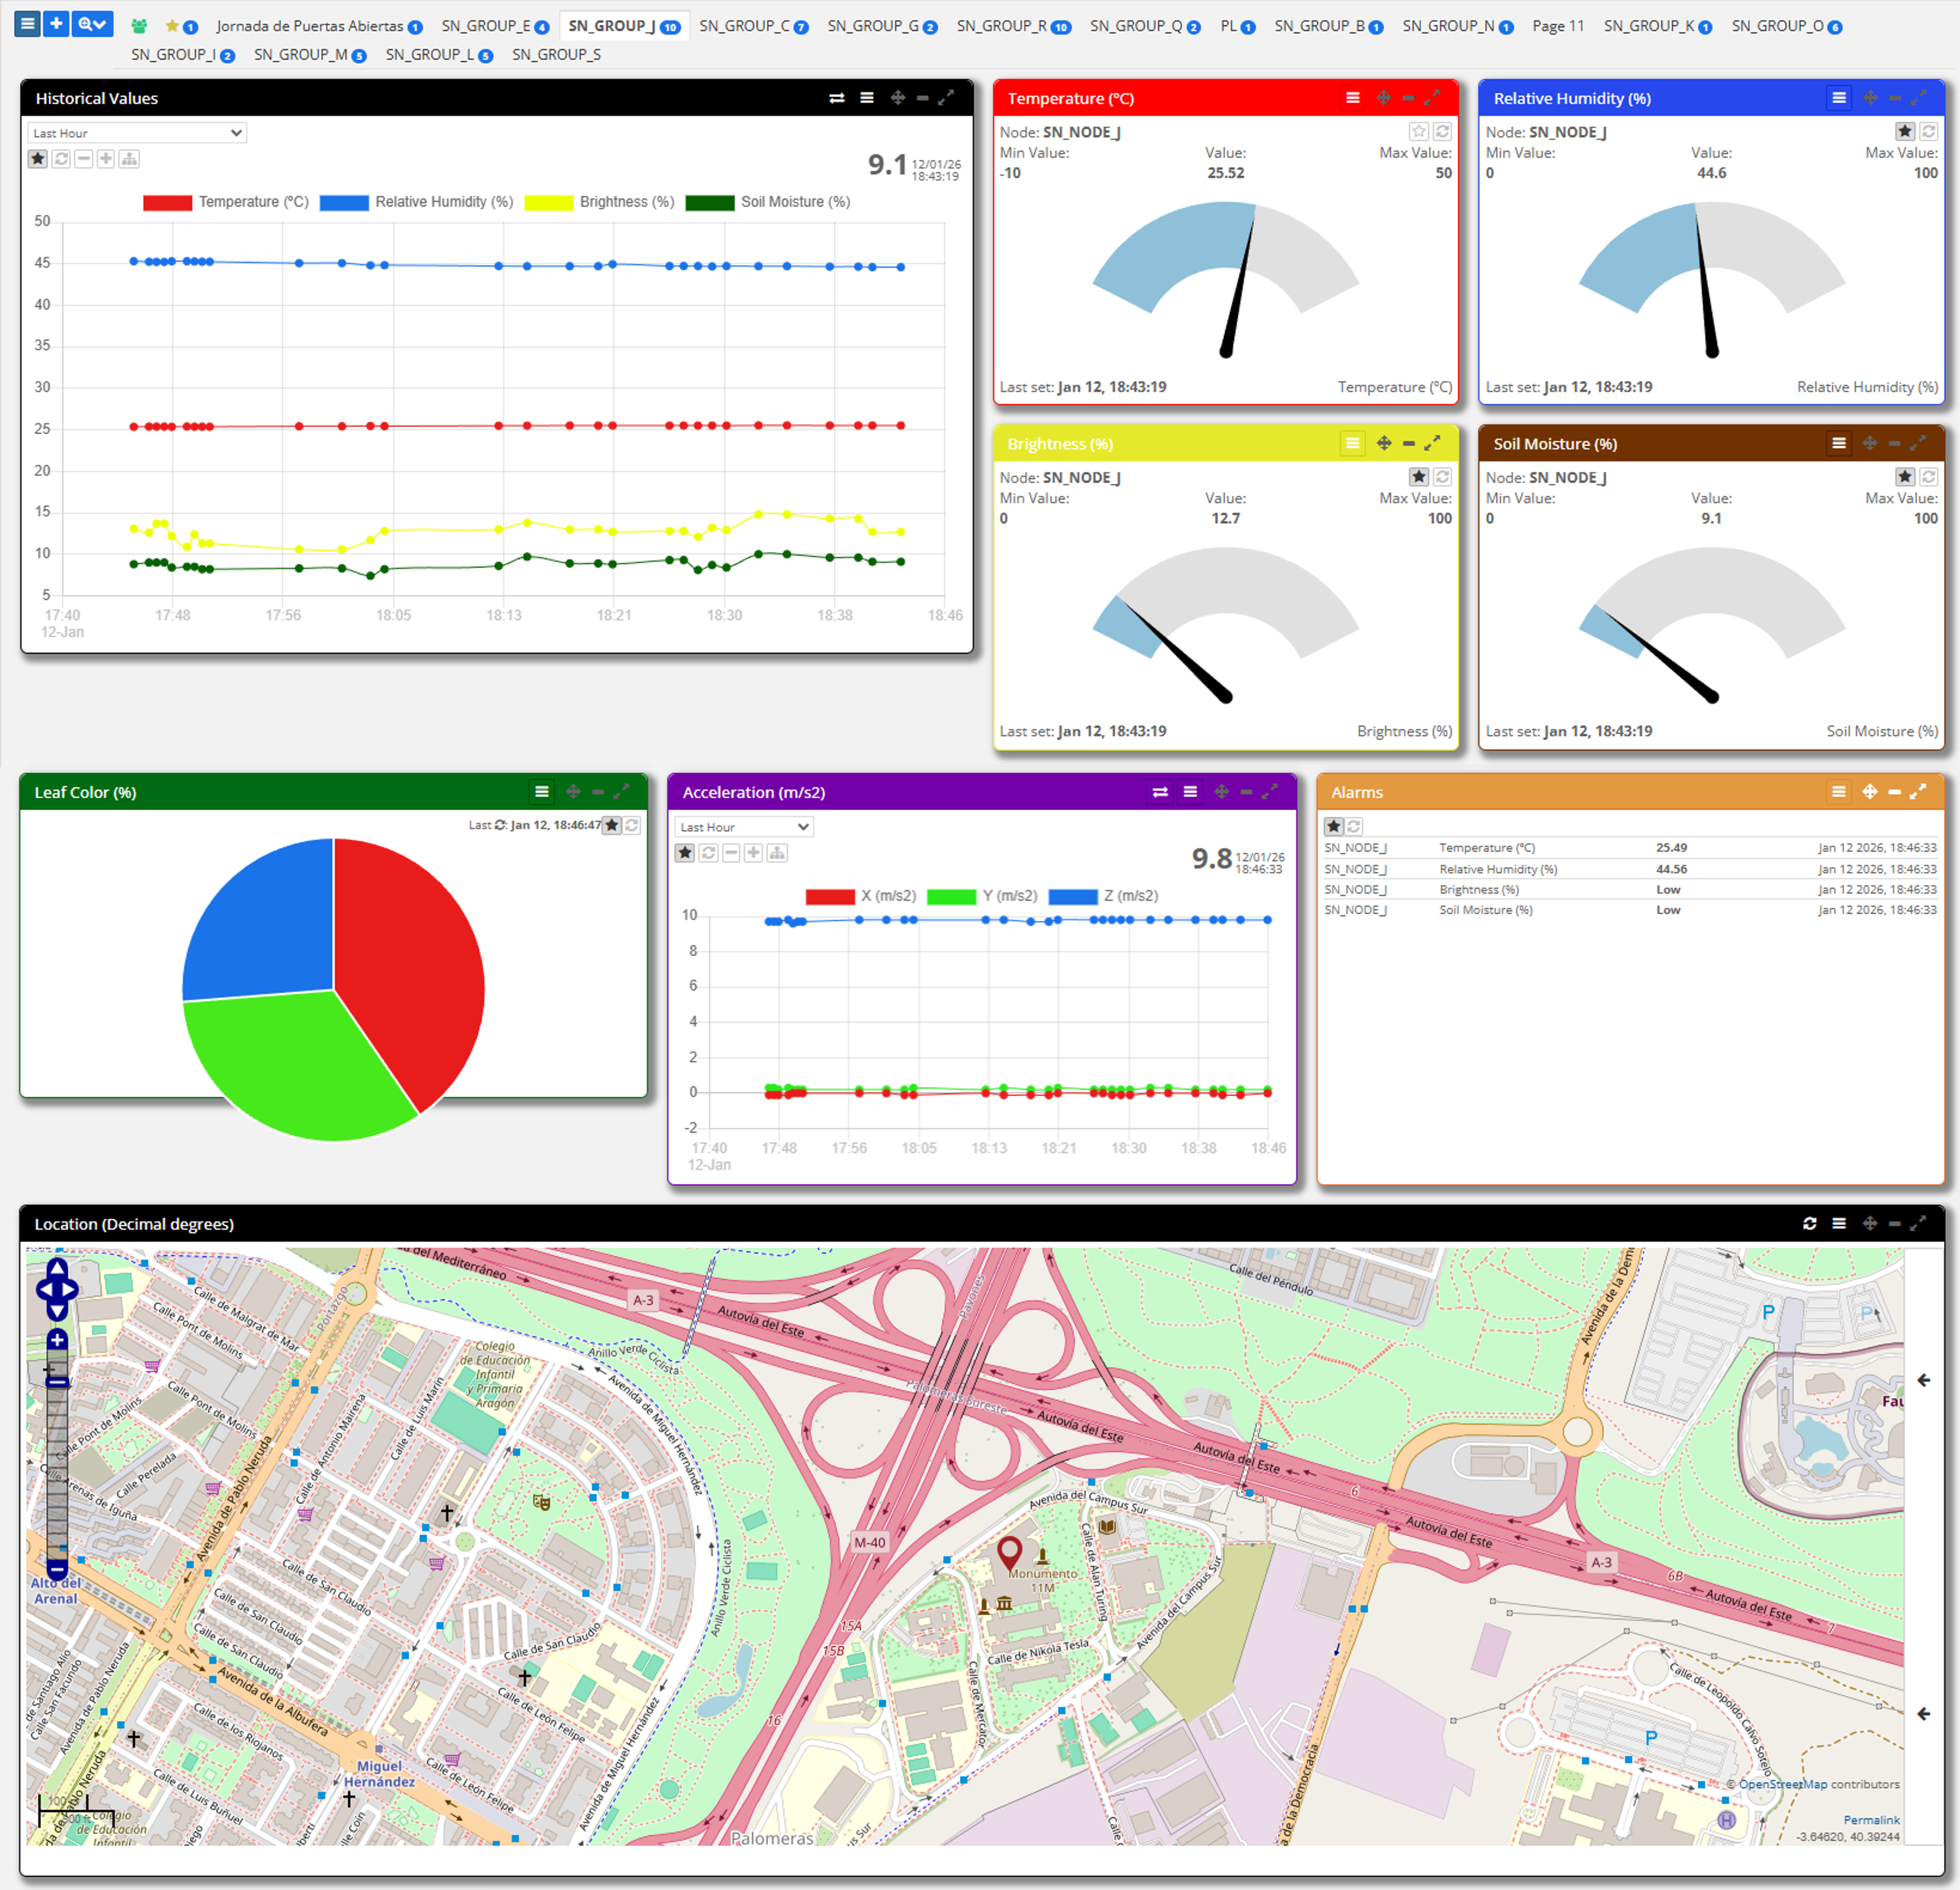
\includegraphics[width=1\textwidth]{images/dashboard.png}
    \caption{ResIoT Dashboard Result}
    \label{fig:dashboard_test}
\end{figure}

\subsection{Mobile Application}

The ResIoT platform features a responsive web-based architecture that allows users to monitor the \textbf{SN\_NODE\_J} system through a mobile interface. As demonstrated in \autoref{fig:mobile}, the \textbf{SN\_GROUP\_J} dashboard automatically adapts its layout to smaller screen sizes, ensuring that all telemetry data remains legible and interactive for remote monitoring.

\begin{figure}[H]
    \centering
    \includegraphics[width=0.3\textwidth]{images/movil.jpeg}
    \caption{Mobile Application View}
    \label{fig:mobile}
\end{figure}

\subsection{\acrshort{RGB} Commands}

The ResIoT platform facilitates bidirectional communication, allowing the user to send \textbf{downlink} commands to the \textbf{SN\_NODE\_J} device to control its integrated \acrshort{RGB} \acrshort{LED}. This process is initiated through the "Node Downlink" interface, where the specific \textbf{DevEUI} and the \gls{LoRaWAN} gateway (\texttt{Building 8 - Roof}) are selected to route the message. As illustrated in Figure \ref{fig:command}, the user inputs the desired color command (in this case, "Green") as the data payload to be transmitted over the \textbf{EU868} network.

\begin{figure}[H]
    \centering
    \includegraphics[width=0.4\textwidth]{images/command.jpeg}
    \caption{Command Sent}
    \label{fig:command}
\end{figure}

Once the command is issued, the platform provides a \textbf{Command Result} log (\autoref{fig:command_result}) to confirm the execution of the request. This log details critical transmission metadata, including the \textbf{AppEUI}, the timestamp of the event, and the specific communication connector utilized.

\begin{figure}[H]
    \centering
    \includegraphics[width=0.5\textwidth]{images/command_result.jpeg}
    \caption{Command Result}
    \label{fig:command_result}
\end{figure}

The physical result of this automation is shown in \autoref{fig:led_result}, where the \gls{LoRaWAN} end-node receives the downlink packet and updates the state of its hardware. The integrated \acrshort{RGB} \acrshort{LED} on the breadboard illuminates in \textbf{green}, matching the issued command.

\begin{figure}[H]
    \centering
    \includegraphics[width=0.15\textwidth]{images/led.jpeg}
    \caption{\acrshort{LED} Result}
    \label{fig:led_result}
\end{figure}


\subsection{CPP Check}

Static code analysis was performed on the project's modules using CPPcheck with a GitHub Action. As illustrated in \autoref{fig:cppcheck}, the analysis yielded a limited number of warnings. The majority of these notifications arise from missing Zephyr-specific libraries. This is a direct result of the GitHub Actions environment lacking a comprehensive Zephyr build context and the necessary toolchain or board support packages. 

Furthermore, while CPPcheck identifies several unused functions, this is expected behavior given that the modules are designed as general libraries rather than exclusive components of this specific system. Ultimately, no critical defects were identified, and the existing warnings do not compromise the functional integrity of the codebase.

\begin{figure}[H]
    \centering
    \includegraphics[width=1\textwidth]{images/cppcheck.png}
    \caption{Cppcheck Result}
    \label{fig:cppcheck}
\end{figure}